\chapter{Particle Filters}
\label{sec:Particle Filter}
\section{Introduction}
Particle filters, a type of Sequential Monte Carlo (SMC) method,
are a powerful method for estimating the posterior probability distribution
 of parameters given a timeseries of measurements. Unlike Markov 
Chain Monte Carlo (MCMC) estimation, particle filters are designed for 
time-varying random variables. The idea behind particle filters is
similar to Kalman Filters; however, unlike Kalman Filters,
distributions are stored as an empircal distribution rather than 
as the first two moments of a Gaussian. Thus, particle filters are 
preferred when the model is nonlinear, and non-gaussian. This section
is largely based on Arulampalam et al. and Thrun et al. \cite{Arulampalam2002a, 
thrun2008probabilistic}.

\section{Model}
\label{sec:Particle Filter Model}
The idea of the particle filter is to build an empirical distribution
out of a large number of parameter sets, called particles. Each
particle contains all the parameters and states needed to propagate
the model forward.  The particle filter begins with a wide distribution 
(called the Prior Distribution)
of possible particles and then, as measurements come in, weights 
particles based on the quality of their output estimates. Thus parameter sets 
that tend to give good estimations of the measurements get weighted higher
than parameter sets that give poor estimates. Although the reliance on
a prior distribution could be problematic, when the system being modeled
has physical meaning, establishing reasonable ranges for parameters may be 
quite easy. Optimizing the prior distribution can be more difficult,
unless the system has been extensively studied.

Suppose a set or stream of measurements at discrete times are given, 
$\{Y_k, k = 1, 2, 3, ... K\}$, where $K$ may be infinite. 
Let $k$ denote a time index and $t_k$ define the continuous
time of index $k$.
Suppose also that there is a hidden set of state variables,
$X(t)$ that drives the value of $Y(t)$. Throughout this section
$X_k$ will identify $X(t_k)$. The goal of the particle filter is to estimate the 
distribution of the
true parameters $\Theta$ that dictates the movement of $X(t)$.
The model also permits random motion in $X(t)$, so the 
particle filter also estimates the distribution of $X(t)$.
The only difference between the members of parameter vector
$\Theta$ and those of $X(t)$ is that the members of
$\Theta$ have no known update equation. Members of both vectors
are permitted to have some noise, although this
may not be explicitly stated in the model. The generic, continuous, nonlinear
system definition is shown in \autoref{eq:GenericNonlinear}.

\begin{eqnarray}
\dot{X}(t) = f(t, X(t), u(t), \theta, \nu_x) \nonumber \\
Y(t) = g(t, X(t), u(t), \theta, \nu_y)
\label{eq:GenericNonlinear}
\end{eqnarray}

$X(t)$ is vector of state variables, $\Theta$ is a vector of system
constants, $u(t)$ is an input, $Y(t)$ the observation, and
$\nu_x$ and $\nu_y$ are random variates. Although any of these
variables could be a vector, for the sake of simplicity only
$\Theta$ and $X(t)$ will be considered as such. 

I will also make a few  simplifying assumptions for this work. 
First, the systems are assumed to be 
time invariant. This 
assumption is based on the idea that if you paused the system for $\Delta t$
seconds, when unfrozen the system would continue as if nothing happened. 
Few biological systems are predictable enough for them to be summarized
by a time varying function, least of all the brain. While heart beats are certainly
periodic and have an effect on the \ac{BOLD} signal, the period varies too much
for the system to be considered varying with time. 
Next, it was assumed that input cannot directly
influence the output, which in the case of the \ac{BOLD} signal is a good assumption.
Finally, because the only difference between the members of $X(t)$ and 
$\Theta$ is an update function, from now on $X$ will encapsulate
$\Theta$. The assumptions allow for a simplified version of the
state space equations:

\begin{eqnarray}
\dot{X}_k &=& f(X_{k-1}, u_k, \nu_x)
\label{eq:stateass}\\
Y_k &= &g(X_k, \nu_y)
\label{eq:measass}
\end{eqnarray}

\section{Sequential Importance Sampling}
The goal of the particle filter is to evolve an empirical distribution 
$P(x_k | u_{0:k}, Y_{0:k})$,
that asymptotically approaches the true probability distribution $P(X_k | u_{0:k})$.
Note that capital $X$ will be used as the actual realizations of 
the state variable, whereas $x$ will denote estimates of $X$.
Additionally, the notation $a:b$ indicates the set $[a,b]$,
as in $u_{a:b}$, which would indicate all the inputs from time $a$ to time $b$.
Considering the noise present in $X$,
 $P(X_k | u_{0:k})$ is not a single true value but probability distribution. 

To begin, the particle filter must be given a prior distribution, from
which the initial $N_p$ particles are drawn. A particle contains a weight
as well as an estimate of $X_k$, which as previously mentioned, contains every
variable needed to run the model. Then the prior is generated from a 
given distribution, $\alpha(X)$, by:

\begin{equation}
\{[x^i_0,w^i] : x^i_0 \sim \alpha(X), w^i = \frac{1}{N_p}, i \in \{1, 2, ... , N_p\} \}
\end{equation}

where $N_p$ is the number of particles or points used to describe the prior 
using a Mixture \ac{PDF}. 
Note that any exponents will be explicitly labeled as such, to avoid confusion with
the particle numbering scheme. 

Therefore, after the particles have been generated they should approximate $\alpha(X)$:

\begin{equation}
\alpha(X) \approx P(x_0) = \int_{-\infty}^{\infty}
    \sum_{i=0}^{N_p} w^i\delta(X - x^i_0 ) dx
\end{equation}
where $\delta(x-x_0)$ is 1 if and only if $x = x_0$ 
(the Kronecker delta function).

If a flat prior is 
preferred, then each particle's weight could be scaled to the reciprocal of the
density at the particle: 
\begin{equation}
w^i = \frac{1}{\alpha(x^i_0)}
\end{equation}
Whether or not to flatten the prior is a design decision. The reason this might 
be preferred over a direct
uniform distribution is that the distribution width will inherently scale 
for increased particle counts although some distributions
flatten out better than others. Either way, $\alpha(X)$ must be
wide enough to incorporate any posterior that arises. If the prior is
not sufficiently dense, the particle filter may be able to compensate, if it is
not sufficiently wide the particle filter won't converge. 

\subsection{Weighting}
For all the following areas, the probabilities implicitly depend on $u_{0:k}$, 
so those terms are left off for simplicity.

Whenever a measurement becomes available it permits refinement of the
posterior density.
This process of incorporating new data is called sequential importance sampling,
and eventually allows convergence. The weight is defined as
\begin{equation}
w^i_k \propto \frac{P(x^i_{0:k} | y_{0:k})}{q(x^i_{0:k} | y_{0:k})}
\label{eq:weightfunc}
\end{equation}
where $q$ is called an \emph{importance density}. The importance density
is the density of the points, thus by dividing by this value, the weight
should not depend on the location of the estimation points, but rather
only on $P(x^i_{0:k} | y_{0:k})$, the probability of that particle
being correct given all the measurements up to time $k$. 
Note that if there is a distant peak in
the posterior that $q$ does not have support points in, there will 
be quantization errors, and that part of the density cannot be modeled. 
This is why it is absolutely necessary that $q$ fully covers 
$P(x^i_{0:k} | y_{0:k})$.

It is helpful
to consider how the importance density affects the initial distribution. 
In the initial distribution, the weights are all the same; and for
the sake of argument, let them all be scaled up to 1. Then
\begin{equation}
w^i_k q(x^i_{0:k} | y_{0:k}) = q(x^i_{0:k} | y_{0:k}) = P(x^i_{0:k} | y_{0:k})
\end{equation}
the estimated probability, $P(x^i_{0:k} | y_{0:k})$ depends only on the 
way the particles are distributed. As new measurements are incorporated,
the weight will accumulate probabilities through time, which will be discussed
next. 

\subsection{Calculating Weights}
To calculate the weight of a particular particle, it is necessary to 
calculate both $q(x^i_{0:k} | y_{0:k})$ and $P(x^i_{0:k} | y_{0:k})$.
Note that $q(x^i_{0:k} | y_{0:k})$ may be simplified by assuming that 
$y_k$ doesn't contain any information about $x_{k-1}$. Technically this 
could be false; since later measurements may shed light on currently hidden
changes in $x$, however in this work it is a good assumption because the
input does not immediately effect the \ac{BOLD} signal. 
\begin{equation}
q(x^i_{0:k} | y_{0:k}) = q(x^i_{0:k} | y_{0:k-1})
\label{eq:QAssump}
\end{equation}
The choice of the importance density is another design decision; however
it is common to use the integrated state equations. 
Although other importance density functions exist; for the particle filter
used here, the standard importance density will be used: the model
prior.
\begin{equation}
q(x_k | x_{k-1}, y_{0:k}) =  P(x_k | x_{k-1})
\label{eq:ImportanceDensity}
\end{equation}
This choice for importance density is conventient since its simply 
the set of particles propagated
forward in time using the state equations. Additionally it makes
updating weights simple, as seen later in \autoref{eq:weightevolve}.

The $q(x^i_{0:k} | y_{0:k})$ may then be simplified:
\begin{equation}
\begin{array}{cclr}
q(x_{0:k} | y_{0:k}) & = & q(x_k | x_{0:k-1}, y_{0:k})q(x_{0:k-1} | y_{0:k}) &  \\
& = & q(x_k | x_{0:k-1}, y_{0:k})q(x_{0:k-1} | y_{0:k-1})  & \text{[\autoref{eq:QAssump}]} \\
& = & q(x_k | x_{k-1}, y_{0:k})q(x_{0:k-1} | y_{0:k-1})  & \text{[Markov Property]}\\
& = & P(x_k | x_{k-1})q(x_{0:k-1} | y_{0:k-1})  & \text{[\autoref{eq:ImportanceDensity}]}
\end{array}
\end{equation}

Calculating $P(x_{0:k} | y_{0:k})$ is a bit more involved. 
First, using the assumption that the distribution of $y_k$ is 
fully constrained by $x_k$, and that $x_k$ is similarly fully 
constrained by $x_{k-1}$, I make the assumptions that:
\begin{eqnarray}
P(y_k | x_{0:k}, y_{0:k-1}) &=& P(y_k | x_k) \nonumber \\
P(x_k | x_{0:k}, y_{0:k-1}) &=& P(x_k | x_{k-1})
\label{eq:MarkovProperty}
\end{eqnarray}
These are of course just re-statements of the state equations assumed 
by \autoref{eq:stateass} and \autoref{eq:measass}.

Additionally, for the particle filter $y_k$ and $y_{0:k-1}$ are 
constant across all particles, thus $P(y_k| y_{0:k-1})$ can
be dropped when the equality is changed to a proportion. 
Using these properties, $P(x^i_{0:k} | y_{0:k})$ may be broken up as follows 
(primarily using Bayes' Theorem):
\begin{equation}
\begin{array}{lclr}
P(x_{0:k} | y_{0:k}) & = & \frac{P(y_{0:k}, x_{0:k})}{P(y_{0:k})} & \\
 & = & \frac{P(y_k, x_{0:k} | y_{0:k-1}) \cancel{P(y_{0:k-1})}}{P(y_k | y_{0:k-1}) \cancel{P(y_{0:k-1})}} & \\
 & = & \frac{P(y_k| x_{0:k}, y_{0:k-1}) P(x_{0:k} | y_{0:k-1})}{P(y_k | y_{0:k-1}) } & \\
 & = & \frac{P(y_k| x_{0:k}, y_{0:k-1}) P(x_k | x_{0:k-1}, y_{0:k-1}) P(x_{0:k-1} | y_{0:k-1})}{P(y_k | y_{0:k-1})} &  \\
& = & \frac{P(y_k| x_k) P(x_k | x_{k-1}) P(x_{0:k-1} | y_{0:k-1})}{P(y_k | y_{0:k-1})}  & [\text{\autoref{eq:MarkovProperty}}]\\
& \propto & P(y_k| x_k) P(x_k | x_{k-1}) P(x_{0:k-1} | y_{0:k-1}) & [P(y_k|y_{0:k-1}) \text{ is constant}]
 \end{array}
 \label{eq:UpdateBayes}
\end{equation}
Inserting \autoref{eq:ImportanceDensity} and the result of \autoref{eq:UpdateBayes}
into \autoref{eq:weightfunc} leads to:
\begin{eqnarray}
w^i_k & \propto & \frac{P(y_k| x^i_k) \cancel{P(x^i_k | x^i_{k-1})} P(x^i_{0:k-1} | y_{0:k-1})}
                         {\cancel{P(x^i_k | x^i_{k-1})}q(x^i_{0:k-1} | y_{0:k-1})} \nonumber \\
& \propto & w^i_{k-1}P(y_k| x_k) 
\label{eq:weightevolve}
\end{eqnarray}

Thus, by making the following simple assumptions, evolving a posterior
density  requires no knowledge of the noise distribution.
\begin{enumerate}
\item $f(t, x(t), u(t)) = f(x(t), u(t))$ and $g(t, x(t), u(t)) = g(x(t))$ 
\item The prior distribution PDF, $q(x_i(0))$, covers $P(x_i(0))$
\item Markov Property: $P(x_k | x_{0:k-1}) = Pr(x_k | x_{k-1})$
\item $q(x_{0:k-1} | y_{0:k}) = q(x_{0:k-1} | y_{0:k-1})$
\end{enumerate}

From the definition of $w_i$, the algorithm to calculate
an approximation of $P(X(t_k) | Y_{0:k})$ or $P(X(t_k + \delta t) | Y_{0:k})$
is simple. This basic form of the particle filter is given in 
algorithm \autoref{alg:BasicParticleFilter}.

\begin{algorithm}
\caption{Sequential Importance Sampling}
\begin{algorithmic}
\STATE Initialize Particles:
\FOR{$i$ : each of $N_p$ particles }
    \STATE $x^i_0  \sim \alpha(X)$
    \STATE $w^i_0 = \frac{1}{N_p}$
\ENDFOR
\FOR{$k$ : each measurement}
    \FOR{$i$ : each particle }
        \STATE $x^i_k = x^i_{k-1} + \int_{t-1}^t f(x(\tau), u(\tau)) d\tau $
        \STATE $w^i_k = w^i_{k-1}P(y_k | x_k)$
    \ENDFOR
\ENDFOR
\STATE $P(x(t_k+\Delta t)) \approx 
\sum_{i=0}^{N_p} w^i_k \delta\left(x - (x^i_k + \int_{t_k}^{t_k+\Delta t} f(x(\tau), u(\tau)) d\tau) \right)$
\end{algorithmic}
\label{alg:BasicParticleFilter}
\end{algorithm}

\section{Sequential Importance Resampling}
\label{sec:Particle Filter Resampling}
\begin{figure}
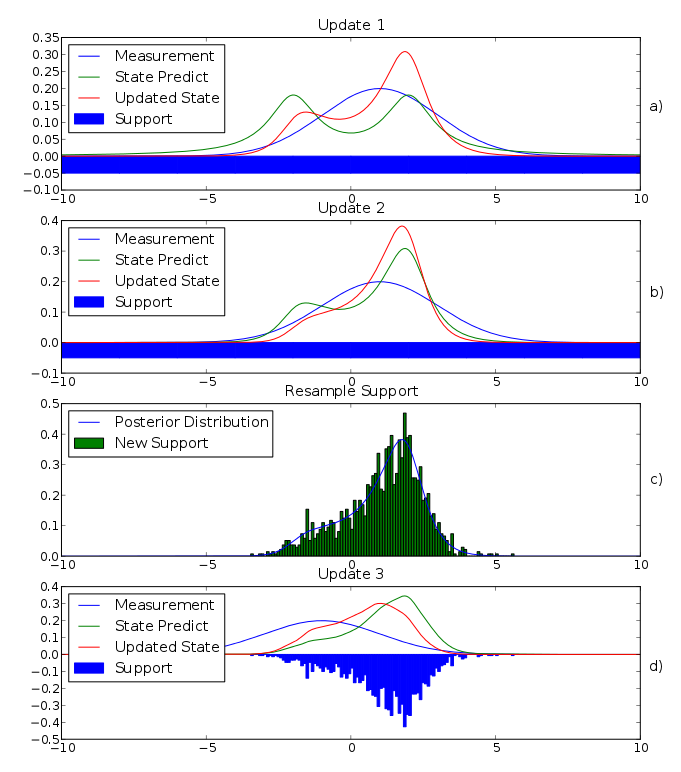
\includegraphics[width=16cm]{images/particle_filter2}
\caption[Example Particle Filter Progression]{a) Initial particle locations
uniformly distributed in [-10, 10], with
weights set to give the State Prediction (green). When a measurement is
received it converted to a distribution approximating uncertainty. This
distribution is then used to alter the weights of the existing particles.
b) Another measurement is applied similar to a), c) Resampling draws
new particles in locations according to the Mixture \ac{PDF} approximated 
by the particle weights. d) Another measurement is applied as before,
but now with non-uniform particle locations.}
\end{figure}

As a consequence 
of the wide prior distribution (required for a proper discretization of a continuous
distribution), a significant proportion of particles will quickly
develop insignificant weights. 
While this does help
describe the tails of the distribution, it means a great deal of computation will be wasted.
Instead, it would be preferable if most of the computation is spent on the most probable regions.
Ideally the computation time spent on tails would be proportional to the actual size of the
tails. In this case particle locations would match the true posterior and all weights would
be equal.  The case where a large number of the weights have become extremely small
is called particle degeneracy. In  Lui et al. 
an ideal calculation of the effective number of particles is found based on the 
particles' true weight \cite{Liu1998}. However, given that only an approximation 
for the true weight 
exists, they also provide a simple heuristic calculation of $N_{eff}$.
\begin{equation}
N_{eff} \approx \frac{\sum_{i=0}^{N_p} w_i}{\sum_{i=0}^{N_p} w_i^2}
\label{eq:neff}
\end{equation}
Unless the prior is particularly accurate,
$N_{eff}$ drops very quickly.  To alleviate particle degeneracy
a common technique known as resampling is often applied. The idea of resampling is to 
draw from the approximate posterior, thus generating a replica of the posterior with 
a better support. Therefore, a new set of particles may be drawn from the empirical
distribution as follows:
\begin{equation}
\hat{x}_j \sim \left(\sum_{i=0}^{N_p} w^i_k\delta(x - x^i_k)\right)
\end{equation}

\begin{algorithm}
\caption{Resampling Algorithm}
\begin{algorithmic}
\STATE Calculate total weight, $W_t = \sum_{i=0}^{N_p} w^i$
\FORALL{$0 < i < N_p$}
    \STATE Draw $V$ from uniform range $[0, W]$
    \STATE $C = W_t$
    \FORALL{$0 < j < N_p$ and $C < V$}
        \STATE $C = C - w^j$
    \ENDFOR
    \STATE Add $[x^j, \frac{1}{N_p}]$ to the new distribution
\ENDFOR
\STATE 
\end{algorithmic}
\label{alg:Resampling}
\end{algorithm}
For infinite particles this new distribution will match the old.
Unfortunately, this isn't the truth in practice: since the support is
still limited to the original particles, the number of \emph{unique} particles can only go down.
This effect, dubbed particle impoverishment can result in excessive quantization
errors in the final distribution. However, there is a solution. Instead of sampling from the
discrete distribution, a smoothing kernel is applied, and particles are drawn from
that distribution. Because it is continuous, particle impoverishment
cannot occur. The easiest way to sample from the continuous distribution is to break the 
re-sampling down into two steps. After calculating an estimate of the scale of the original
distribution, algorithm \autoref{alg:Resampling} is performed. Next, a distribution is generated
based on the variance of the original distributions.
Finally, for each particle in the discretely re-sampled distribution, a sample is drawn from 
the smoothing 
distribution and added to the particle.  The regularization process is defined as:

\begin{equation}
x_i = x_i + h\sigma \epsilon
\end{equation}

Where $h$ is an optional bandwidth, $\sigma$ is the standard deviation such that 
$\sigma \sigma^T = cov(x)$
and $\epsilon$ is drawn from the chosen kernel. The choice of a kernel is
complex, although it has been proven that the optimal kernel for reducing \ac{MSE} between
the original and resampled distributions is 
is the Epanechnikov Kernel \cite{Musso2001a}. However, Musso et al. 
also espoused the usefulness of the Gaussian Kernel, due to the ease
drawing samples from it, which for this work was more important \cite{Musso2001a}.

\begin{algorithm}
\caption{Regularized Resampling Algorithm}
\begin{algorithmic}
\STATE Calculate Covariance, $C$, of empirical distribution, $\hat{x}$
\STATE Find $D$ such that $DD^T = C$
\STATE Resample $\hat{x}$ using algorithm \autoref{alg:Resampling}
\FOR{$0 < i < N_p$}
    \STATE Draw $\epsilon$ from the standard normal, same dimensionality as $X$
    \STATE $x^i = x^i + hD\epsilon$
\ENDFOR
\end{algorithmic}
\label{alg:RegResampling}
\end{algorithm}

Hurzeler et al. demonstrated that if the underlying 
distribution is non-Gaussian, then using the original bandwidth may over-smooth
\cite{Hurzeler1998}.  In reality, over smoothing
will only become an issue if resampling is performed often. Thus
if resampling is performed at every step then this would certainly cause problems.
If the distribution is over-smoothed then the algorithm may not converge as rapidly,
or at all. However, because the bandwidth is still based on particle variance, 
which should decay as particles are ruled out, the particle filter is still able to converge. 
In fact, over-smoothing is preferable
to under smoothing, since over-smoothing simply slows convergence while 
under-smoothing could leave gaps in the distribution.
Moreover, because of the high dimensionality of the \ac{BOLD} model,
and limited measurements, it is helpful to have a broader bandwidth to explore the distribution. 

\begin{algorithm}
\caption{Regularized Particle Filter}
\begin{algorithmic}
\STATE Initialize Particles:
\FOR{$i$ : each of $N_p$ particles }
    \STATE $x^i_0  \sim \alpha(X)$
    \STATE $w^i_0 = \frac{1}{N_p}$
\ENDFOR
\FOR{$k$ : each measurement}
    \FOR{$i$ : each particle }
        \STATE $x^i_k = x^i_{k-1} + \int_{t-1}^t f(x(\tau), u(\tau)) d\tau $
        \STATE $w^i_k = w^i_{k-1}P(y_k | x_k)$
    \ENDFOR

    \STATE Calculate $N_{eff}$ with \autoref{eq:neff}
    \IF{$N_{eff} < N_R$ (recommend $N_R = min(50, .1N_p)$ )}
        \STATE Resample using algorithm \autoref{alg:RegResampling}
    \ENDIF
\ENDFOR

\STATE At $t + \Delta t$, $t \in T$, $P(x(t+\Delta t)) \approx 
\sum_{i=1}^{N_p} w_i(t)\delta\left(x - (x_i(t) + \int_t^{t+\Delta t} f(x(\tau), u(\tau)) d\tau) \right)$
 \end{algorithmic}
 \label{alg:RegularizedParticleFilter}
 \end{algorithm}

Because 
of the potentially wide smoothing factor applied by regularized resampling, performing this
step at every measurement would allow particles a great deal of mobility. Therefore
in this work regularized resampling was only performed when $N_{eff}$ dropped
below 50. Other than the periodic regularized
resampling, the regularized particle filter is identical to the basic sampling
importance sampling filter (SIS). 

With regularized resampling, it is possible to prevent both
particle degeneracy as well as particle impoverishment. 
Note that resampling carries certain risks.  
If for some reason the solution is not covered by the 
new support, the algorithm may not be able to reach the true value. 
The ultimate effect of this regularized resampling is a convergence 
similar to simulated annealing or a genetic algorithm. 
Versions of $x$ that are fit (give good measurements) spawn more children 
nearby which allow for more accurate estimation near points of high likelihood. 
As the variance of the estimated $x$'s decrease, the radius in 
which children are spawned also decreases. Eventually the radius
will approach the width of the underlying uncertainty.

\section{Weighting Function}
Because the distribution of $\nu_y$ in \autoref{eq:measass} is unknown,
it is necessary to choose a distribution for this. This distribution
is important because $\nu_y \sim P(y_k | x(T))$, which is used
for updating weights. Ideally this weighting function would exactly 
match the measurement error in the output. 
While a Gaussian function is the traditional choice, there are other reasonable
distributions, given the nature of the noise present in FMRI.
The choice of this function will be discussed further in \autoref{sec:Methods Weighting Function}.

%\section{Piecewise Example}
%A half wave rectifier takes a \ac{AC} voltage circuit and removes
%the negative half  of the signal. The resulting waveform
%is still not DC, however it is then possible to use a capacitor to 
%smooth the signal into something similar to DC, as shown in \autoref{fig:HalfWaveIO}.
%There are other, more
%complex circuits that convert the negative portion into positive and
%waste less energy but here I will keep the system simple.
%Thus, consider a simple half wave rectifier circuit, shown in 
%\autoref{fig:HalfWaveRectifier}.
%
%The half wave rectifier circuit smoothes the gaps between high voltage
%with a capacitor. Thus, when $u(t)G$ is less than $v_t$, the circuit will 
%discharge the capacitor and maintain a non-zero voltage,
%but when $u(t)G$ is greater than $v_t$, the output voltage will be set
%by $u(t)G$ and the capacitor will charge up. I will assume a simple
%model for all the components, ignoring the complex nonlinear behavior
%that can occur in the components. Also note that the 
%
%\begin{figure}
%\centering
%\begin{circuitikz}[scale=2, american]
%\draw
% (0,0)  node[transformer core] (T) {}
% (T.A1) -- (-1,0)
% (T.A2) -- (-1,-1.05)  to[V, v=$u(t)$] (-1, 0)
% (T.B1) -- (.5, 0) to[D, l=$v_t$] (1.5,0) to[C=$C$] (1.5, -1.05)
% (1.5, 0) -- (2.5, 0) to[R=$Rm$, v=$v_y$] (2.5, -1.05) -- (T.B2) 
% (T.base) node {G}
% (T.B1) to[open, *-*, v=$V_1$] (T.B2); 
%\end{circuitikz}
%\caption{An Example Half Wave Rectifier Circuit, where $G$ is the transformer
%gain, $v_t$ is the activation voltage of the diode, $u(t)$ is the input at time $t$, 
%$C$ is the capacitance, $R$ is the load resistance and $v_y$ is the output voltage}
%\label{fig:HalfWaveRectifier}
%\end{figure}
%
%\begin{figure}
%\centering
%\caption{Example Input/Output of the Half Wave Rectifier}
%\label{fig:HalfWaveIO}
%\end{figure}
%
%Consider the piecewise function in \autoref{eq:example}. 
%As discussed in the \autoref{sec:Particle Filter Model}
%any variable with uncertainty must be part of the state variable. Therefore,
%even though $G$, $C$, $R_m$ and $V_t$ are constants, they are still
%included in the state variable: $X(t) = \{G, V_t, C, R_m, v_y\}$. 
%
%\begin{equation}
%v_y(t)  = f(v_y(t-1, u(t)) =  \begin{cases} 
%        u(t)G & \text{ if }  u(t)G-v_y \ge V_t\\
%        v_y(t-1)\left(1 - \frac{\delta t}{R_mC}\right) & \text{ if }  u(t)G-v_y < V_t
%    \end{cases} 
%\end{equation}
%
%To run the particle filter is easy, since there exists 
%a recursive definition of the dynamic state variable, $v_y$.
%To start with, an initial distribution must be used; which for
%this case will be:
%Gaussian seems like a good idea, all the static state variables are strictly
%positive and thus not well suited to the Gaussian. Thus, instead the prior 
%will start with a Gamma distribution. The gamma is defined as follows:
%
%\begin{equation}
%X \sim Gamma(k, \theta) \rightarrow f(x) = x^{k-1}\frac{e^{-x/\theta}}{\theta^k\Gamma(k)}
%\end{equation}
%
%where $\Gamma$ is the gamma function.
%The margin for error is decided by the weighting function, which
%will be defined as $W(V_y, v_{yi})$, where $V_y$ is the actual measurement, $v_y$ is the 
%estimate based on all the particles, and 
%$v_{yi}$ is the estimate by a particular ($i^{th}$) particle. The choice of this function is difficult,
%and although the Gaussian is typically used, in practice I found the exponential helpful
%in preventing particle deprivation. The algorithm is then,
%
%\begin{algorithmic}
%\STATE Initialize $N_p$ Particles:
%\FOR{$i$ in $N_p$}
%    \STATE $G \sim Gamma(\frac{\mu^2_G}{\sigma^2_G}, \frac{\sigma^2_G}{\mu_G})$
%    \STATE $v_t \sim Gamma(\frac{\mu^2_{v_t}}{\sigma^2_{v_t}}, \frac{\sigma^2_{v_t}}{\mu_{v_t}})$
%    \STATE $C \sim Gamma(\frac{\mu^2_C}{\sigma^2_C}, \frac{\sigma^2_C}{\mu_C})$
%    \STATE $R_m \sim Gamma(\frac{\mu^2_R}{\sigma^2_R}, \frac{\sigma^2_R}{\mu_R})$
%    \STATE $v_y = 0$, (Assume the system has been off for a long time)
%    \STATE let $X_i(0) = \{G, v_t, C, R_m, v_y\}$
%    \STATE let $w_i(0) = 1$ or to make a flat prior, $w_i(0) = \frac{1}{Pr(X_i(0))}$ 
%\ENDFOR
%\STATE Run the Filter:
%\FOR{$t$ in Set of Measurement Times}
%    \FOR{$i$ in $N_p$}
%        \STATE $v_{yi}(t) = f(v_{yi}(t-1), u(t))$
%        \STATE (All other members of $X_i(t)$ remain the same)
%        \STATE $w_i(t) = w_i(t-1)W(V_y(t), v_y(t))$
%    \ENDFOR
%\ENDFOR
%\end{algorithmic}
%
%Initially the particles will have the same output, $0$, however, as $u(t)$
%changes, the response of each particle to that input will result in different
%outputs. Particles that have a $v_{yi}$ near $V_y$ will be weighted higher,
%and others farther away will be weighted lower. As the particle filter
%runs, weights will compound converging to a distribution that asymptotically
%approaches the true joint distribution of the $X(t)$.  As I
%mentioned in \autoref{sec:Particle Filter Resampling}, particles with 
%weights approaching zero do not significantly
%contribute to the empirical distribution, so re-sampling will be necessary.

